%
% TX-Pi Handbuch
%
\documentclass[
%  headings=normal,
  paper=A4,
%  oneside,
  ngerman,
  fontsize=12pt,
  parskip=half-,
]{scrbook}
\usepackage[ngerman]{babel}
\usepackage{graphicx, geometry}
\usepackage{booktabs}
\usepackage{listings}
\usepackage{color}
\usepackage{fontspec}
\usepackage{paratype}
\setmainfont{PT Sans}
\setsansfont{PT Sans}
\setmonofont{PT Mono}[Scale=0.88]
\definecolor{listing}{gray}{0.95}
\lstset{
  backgroundcolor=\color{listing}
}
\usepackage[hidelinks]{hyperref}
\hypersetup{
  pdfpagemode = UseNone,
  pdfstartview = FitH,
}

\title{TX-Pi — Handbuch}

\hyphenation{ftDuino}

\begin{document}
\begin{titlepage}
  \vspace*{1cm}
  {\huge\raggedright\textbf{TX-Pi — Handbuch}\par}
  {\vfill\par}
  {\url{https://tx-pi.de}\par}
\end{titlepage}

\tableofcontents

\chapter{Einführung}

Ein TX-Pi ist eine kostengünstige und vor allem flexible und aktuelle Alternative zu einem 
fischertechnik TXT-Controller\footnote{TXT-Controller\par\url{https://www.fischertechnik.de/de-de/produkte/spielen/robotics/522429-txt-controller}} in Kombination mit der fischertechnik 
Community-Firmware\footnote{Community Firmware \url{https://cfw.ftcommunity.de/}}.

Der TX-Pi basiert auf dem Raspberry Pi sowie dem Betriebssystem Raspbian und bietet
diverse Anbindungen an aktuelle und auch als gemeinhin veraltet wahrgenommene fischertechnik Hardware.

Zudem entfaltet der TX-Pi insbesondere in Kombination mit einem ftDuino\footnote{ftDuino \url{https://http://ftduino.de/}} die
gleichen sowie noch mehr Möglichkeiten als derzeit mit offizieller fischertechnik 
Hardware realisierbar. 

Es profitieren insbesondere rechen- und speicherintensive Anwendungen von den 
Möglichkeiten des TX-Pi. Ferner lassen sich aufgrund der Offenheit des
Systems neue Anwendungsbereiche wie KI-Systeme oder die Ansteuerung von Sensoren, 
die von fischertechnik nicht unterstützt werden, erschließen.


\section{Vergleich des TXT-Controller mit dem TX-Pi}

Die Hardware des TX-Pi ist ungleich moderner und leistungsfähiger als die des TXT-Controllers.
Ein TX-Pi ließe sich auch mit einem Raspberry Zero betreiben, jedoch werden 
die leistungsstärkeren Rechner Raspberry Pi 3B und der Raspberry Pi 4 für den Betrieb des TX-Pi empfohlen.

Wie der Tabelle \ref{tab:comparison} zu entnehmen ist, fehlen dem TX-Pi notwendige Ein- und Ausgänge,
um ihn mit fischertechnik Komponenten (Taster, Lichter, Motoren etc.) verbinden zu können.
Hierzu bedarf es weiterer Controller wie beispielsweise den ftDuino oder fischertechnik
Komponenten wie das ROBO Interface oder den Robo LT Controller.

\begin{table}[ht]
\begin{tabular}{lccc}
                      & \textbf{TXT-Controller}   & \textbf{Raspberry Pi 3B}     & \textbf{Raspberry Pi 4} \\
\midrule
CPU                   & TI-AM3359-Sitara & Broadcom BCM2837    & Broadcom BCM2711 \\
Kerne                 & 1                & 4                   & 4 \\
Takt (MHz)            & 600              & 1200                & 1500 \\
Arbeitsspeicher (MB)  & 256 / 128 Flash  & 1024                & 1024 - 4096 \\
USB 2.0               & 1                & 4                   & 2 \\
USB 3.0               & -                & -                   & 2 \\
Display					 & 2.4"'              & 3.2"' - 3.5"'      & 3.2"' - 3.5"' \\
Lautsprecher          & Ja               & Nein                & Nein \\
Motorausgänge         & 4                & -                   & - \\
Eingänge              & 8                & -                   & - \\
Zählereingänge        & 4                & -                   & -
\end{tabular}
\caption{Hardware-Vergleich TXT und TX-Pi}
\label{tab:comparison}
\end{table}


\chapter{Installation}

Jeder Raspberry Pi mit einem aktuellen Betriebssystem (Stretch oder Buster) läßt 
sich in einen TX-Pi verwandeln, indem das Installationsscript heruntergeladen
und ausgeführt wird.

Noch einfacher gelingt die Installation mit einem der Betriebssystem-Images,
die unter \url{https://tx-pi.de/images/} angeboten werden.

\section{Installation via Betriebssystem-Image}
\label{sec:image}

Am einfachsten gelingt die Installation mit einem der Betriebssystem-Images,
die unter \url{https://tx-pi.de/images/} abrufbar sind.

Die Betriebssystem-Images werden anhand von Touchscreen-Eigenschaften 
angeboten, jedoch läßt sich ein TX-Pi auch ohne ein Display
betreiben.

Sofern keines der Images auf die verwendete Konfiguration zutrifft, 
sollte das Image "`TX-Pi mit Waveshare 3.5"' Typ A Display"'  heruntergeladen werden. 
Dieses unterstützt sowohl Installationen ohne einen 
Touchscreen als auch andere Konfigurationen wie das Waveshare
4"' Display.

Zum Kopieren des Archives auf eine SD-Karte kann plattformübergreifend
das Programm balenaEtcher\footnote{Etcher \url{https://www.balena.io/etcher/}} verwendet werden.
Dazu muss das entsprechende Image via "`\texttt{Select image}"' ausgewählt
werden. Das Image muss dazu nicht entpackt werden, es kann auch das
Zip-Archiv selektiert werden. Danach wird mit der Schaltfläche "`\texttt{Select drive}"'
das Laufwerk mit einer SD-Karte ausgewählt. Hier sollte mit Bedacht vorgegangen
werden, da die Daten auf dem ausgewählten Laufwerk unwiderruflich gelöscht
werden, sobald man den Prozess mit der Schaltfläche "`\texttt{Flash!}"' angestoßen
hat.
\clearpage

\begin{figure}[ht]
\centering
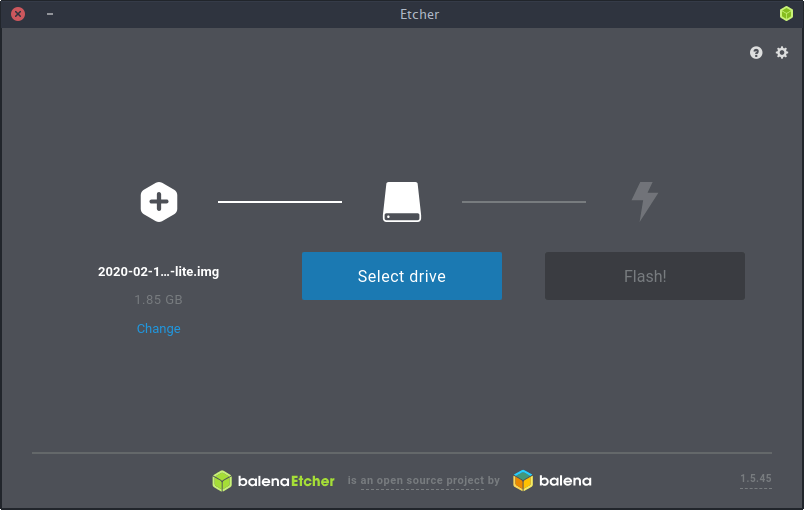
\includegraphics[scale=0.45]{images/etcher.png}
\caption{balenaEtcher zum Flashen einer SD-Karte}
\end{figure}

Die vorbereitete SD-Karte kann nun in den Raspberry Pi eingelegt
und der Rechner gebootet werden.

Nach ein paar automatischen Vorbereitungen sowie einem Reboot wird 
die Benutzungsoberfläche des TX-Pi geladen. 

\subsection{Einrichtung von SSH und WLAN}
Erfahrene Anwender können nach dem Kopieren des Images (siehe \ref{sec:image}) noch die Einrichtung
des SSH-Servers auf dem TX-Pi forcieren, indem im Verzeichnis \texttt{/boot/}
eine (leere) Datei \texttt{ssh} abgelegt wird. 

\textbf{Achtung}: Es sollte nach dem ersten Hochfahren des TX-Pi
das Passwort des Users \texttt{pi} geändert werden!

Einloggen via SSH nach dem ersten Booten des TX-Pi (Passwort: \texttt{raspberry})
\begin{lstlisting}
ssh -l pi IP_ADRESSE_DES_TX_PI
\end{lstlisting}

Passwort ändern
\begin{lstlisting}
pi@raspberrypi:~ $ passwd
\end{lstlisting}

Ferner kann auch eine WLAN-Verbindung auf dem TX-Pi eingerichtet 
werden, indem im Verzeichnis \texttt{/boot/} eine Datei 
\texttt{wpa\_supplicant.conf} abgelegt wird. 
Diese sollte folgenden Inhalt haben:
\begin{lstlisting}
ctrl_interface=DIR=/var/run/wpa_supplicant GROUP=netdev
update_config=1
country=DE

network={
    ssid="HIER_DIE_KENNUNG_DES_NETZWERKES"
    psk="HIER_DAS_PASSWORT_DES_NETZWERKES"
}
\end{lstlisting}

Beide Dateien sind optional, das Starten des SSH-Servers und
die Konfiguration des WLAN kann auch später in der Benutzungsoberfläche
des TX-Pi vorgenommen werden, vgl. Kapitel \ref{chapter:config}


\section{Installation mittels des TX-Pi-Scripts}

Sofern eine existierende Raspbian-Lite Version in ein TX-Pi
überführt werden soll, muss man sich (bspw. via SSH) auf dem 
Rechner einloggen und dann das Installationsscript via
\begin{lstlisting}
wget https://tx-pi-setup.sh
\end{lstlisting}
herunterladen.

Das Script kann anschließend mittels
\begin{lstlisting}
sudo bash ./tx-pi-setup.sh
\end{lstlisting}
ausgeführt werden.

Das Script setzt eine Internetverbindung voraus, da diverse Pakete geladen und
installiert werden.

Das Script nimmt einen Waveshare 3.2"'-Touchscreen an und installiert
dementsprechende Treiber, welche auch einen Betrieb ohne den vorgenannten
Touchscreen zulassen.

Das Script bietet aber auch die Option, das verwendete Display zu 
konfigurieren, hierzu ist ein zusätzlicher Parameter, vgl. Tabelle \ref{tab:display_opt},
notwendig.

\begin{table}[ht]
\begin{tabular}{ll}
Parameter & Display \\
\midrule
          & Waveshare 3.2"' \\
LCD35     & Waveshare 3.5"' Typ A \\
LCD35B    & Waveshare 3.5"' Typ B (IPS Display)\\
LCD35BV2  & Waveshare 3.5"' Typ B Version 2 (IPS Display rev. 2)\\
\end{tabular}
\caption{Optionen für das Display}
\label{tab:display_opt}
\end{table}

Für einen Touchscreen 3.5"' Typ A ist das Installationsscript somit wie folgt aufzurufen:
\begin{lstlisting}
sudo bash ./tx-pi-setup.sh LCD35
\end{lstlisting}

Der Treiber für das Typ A Display eignet sich i.d.R. auch für andere
Displays, wie das Waveshare 4"'.


Nach dem Starten des Scripts wird automatisch das bestehende Betriebssystem aktualisiert
sowie diverse Pakete installiert. 

Die Installation dauert je nach der verwendeten Raspbian-Version ca. 30 Min. Unter Stretch/Raspbian 9.x
ggfs. etwas länger, da mehr Pakete aktualisiert werden müssen.

Anschließend wird der Raspberry Pi automatisch neu gestartet und die Benutzungsoberfläche des TX-Pi erscheint nach dem Neustart.

\begin{figure}[h]
\centering

\includegraphics[scale=0.5]{images/gui-start.png}
\caption{TX-Pi GUI}
\end{figure}


\chapter{Weboberfläche}

Nach der Installation steht auch die Weboberfläche des TX-Pi zur Verfügung.
Im Browser ist sie unter \texttt{http://IP\_DES\_TX-PI/} erreichbar.

Die IP-Adresse kann i.d.R. im Router nachgeschlagen, oder aber
vom TX-Pi angezeigt werden, siehe dazu \ref{sec:ipaddr}.

Über die Oberfläche ist auch der VNC-Client erreichbar, über den
sich der TX-Pi auch ohne Touchscreen im Browser bedienen lässt.

\begin{figure}[h]
\centering
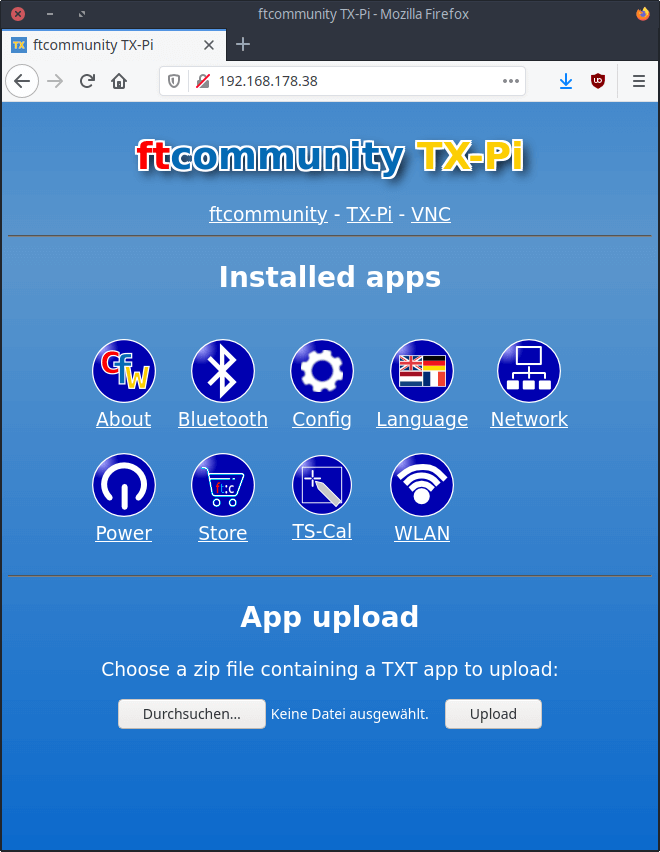
\includegraphics[scale=0.35]{images/browser.png}
\caption{Weboberfläche des TX-Pi}
\end{figure}


\chapter{Konfiguration}
\label{chapter:config}

\section{Generelle Konfiguration}
\label{sec:config}

Der TX-Pi kann u.a. über die Config-App konfiguriert werden. Die App befindet sich
in dem Verzeichnis "`System"'.

\begin{figure}[h]
\centering
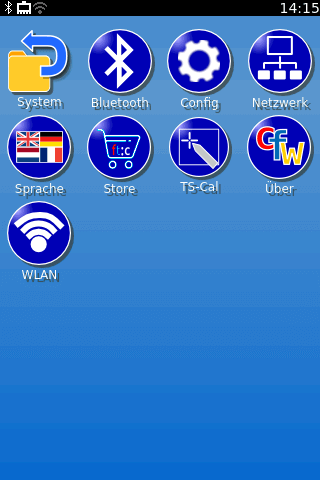
\includegraphics[scale=0.4]{images/gui-system.png}
\caption{Verzeichnis System}
\end{figure}

Über das Menü lassen sich die Konfigurationsmöglichkeiten wählen.

\begin{figure}[h]
\centering
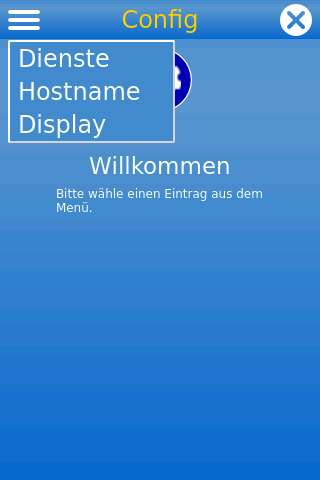
\includegraphics[scale=0.4]{images/config-menu.png}
\caption{Konfigurationsmenü}
\end{figure}


Unter dem Menüpunkt "`Dienste"' lässt sich u.a. der SSH-Server ein- und ausschalten,
sowie der Kamera-Port auf dem Raspberry Pi aktivieren. 

\begin{figure}[ht]
\centering
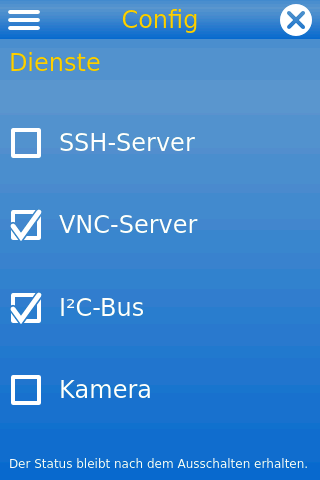
\includegraphics[scale=0.4]{images/config-services.png}
\caption{Konfiguration von Diensten}
\end{figure}

Sofern der SSH-Server aktiviert wurde, sollte das Standardpasswort "`raspberry"'
für den Nutzer "`pi"' geändert werden. Dies ist generell empfehlenswert, unabhängig vom
Status des SSH-Servers.

Eine Konfigurationsseite für das Display wird ebenfalls angeboten. Hier kann die 
Rotation des Displays verändert oder der SPI-Takt erhöht werden, was zu einer
flüssigeren Ausgabe auf dem Bildschirm führen kann. Allerdings sollten die 
Werte hier nur mit Bedacht geändert werden, ansonsten könnte es passieren, dass 
der Touchscreen nicht mehr bedienbar ist. Es bietet sich an, zuvor den SSH-Server und /
oder VNC-Server zu aktivieren, so dass man noch auf den TX-Pi zugreifen kann, wenn das
Display ausfällt.


\section{WLAN-Konfiguration}
\label{sec:wlan}

Über die WLAN-App, die ebenfalls im Verzeichnis "`System"' zu finden ist, kann das
Netzwerk ausgewählt und konfiguriert werden.

Sofern die App nach dem Starten keine verfügbaren Netzwerke anzeigt, kann die App
geschlossen und wieder geöffnet werden. Spätestens dann sollten die verfügbaren
Netze angezeigt werden.

\begin{figure}[ht]
\centering
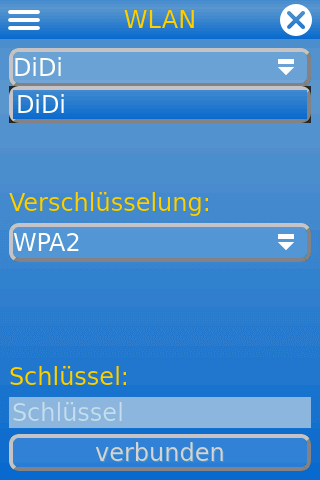
\includegraphics[scale=0.4]{images/wlan.png}
\caption{WLAN-Konfiguration}
\end{figure}


\chapter{Installieren von Apps}

\section{App-Stores}

Am komfortabelsten lassen sich weitere Apps über die App-Stores
installieren. Der TX-Pi hat bereits drei App-Stores installiert;
hierzu gehört neben dem Store der Community Firmware auch ein 
TX-Pi-Store in der Anwendungen zu finden sind, die aufgrund
der schwächeren Hardware nicht auf einem TXT-Controller laufen
oder aber auf den TX-Pi angepasst sind und somit den TXT-Controller
nicht unterstützen.

In der Regel sollte man bei der Anwendungsentwicklung jedoch
darauf achten, dass die App unabhängig von der dem Endgerät TX-Pi
funktioniert.

Die Store-App bietet einen einfachen Zugriff auf die Stores; diese
App befindet sich im Verzeichnis "`System"'. Nach dem Start wird
der Store der Community-Firmware angezeigt, vgl. Abbildung \ref{img:store}

\begin{figure}[ht]
\centering
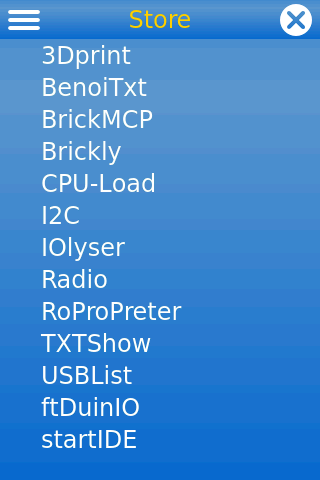
\includegraphics[scale=0.4]{images/store.png}
\caption{App-Store}
\label{img:store}
\end{figure}


Zu den anderen Stores gelangt man über das Menü. 

\begin{figure}[ht]
\centering
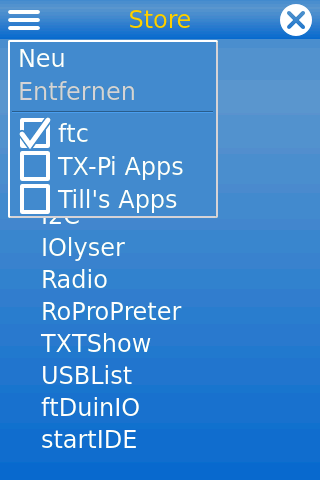
\includegraphics[scale=0.4]{images/store-menu.png}
\caption{App-Store Menü}
\end{figure}

Nachdem eine App selektiert wurde, wird eine Beschreibung der
App angezeigt. Über das Menü kann man dann die App installieren.

\begin{figure}[ht]
\centering
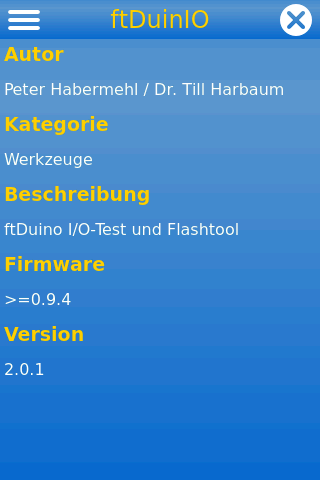
\includegraphics[scale=0.4]{images/store-app-selected.png}
\caption{Beschreibung einer App}
\end{figure}

Über das gleiche Menü lässt sich die App auch wieder deinstallieren
oder aktualisieren.

\begin{figure}[ht]
\centering
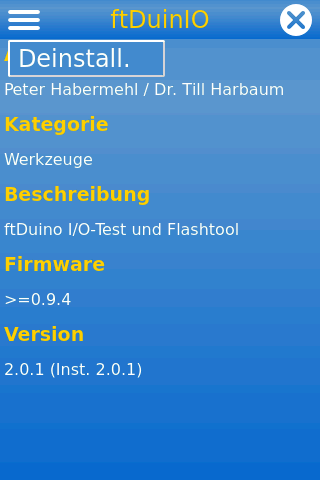
\includegraphics[scale=0.4]{images/store-app-deinstall.png}
\caption{App deinstallieren}
\end{figure}

\section{Weboberfläche}

Als zweite Möglichkeit bietet sich die Weboberfläche an, über die
Apps auf den TX-Pi geladen werden können. In diesem Falle muss die
App in einem Zip-Archiv vorliegen.
Diese Option ist vor allem für eigene Entwicklungen sinnvoll, die
nicht in einem App-Store vorliegen oder sich in einem frühen Entwicklungsstadium
befinden, so dass eine Veröffentlichung in einem Store nicht sinnvoll ist.


\chapter{Gehäuse}

Ein Raspberry Pi mit der Community-Firmware bietet zwar schon einige
Vorteile, aber er lässt noch nicht mit den fischertechnik Bausteinen 
verbauen. 

Hierzu bietet das Projekt einige Gehäusevarianten an, die es erlauben, den 
Rechner in die eigenen fischertechnik Modelle einzubauen.

\begin{figure}[ht]
\centering
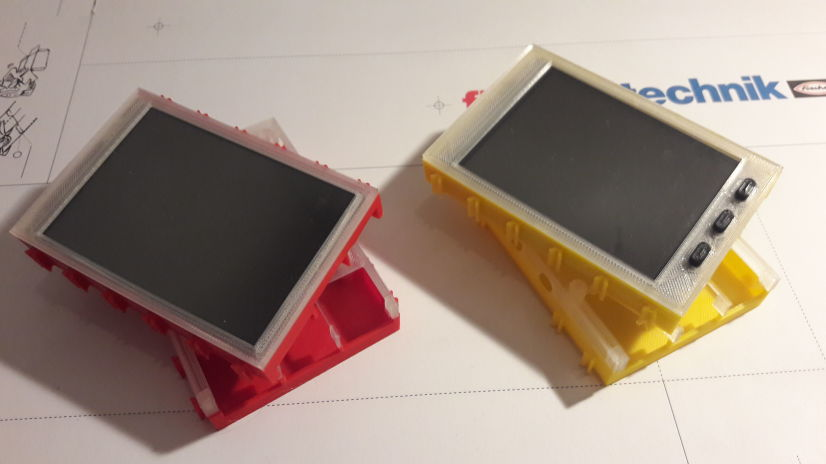
\includegraphics[scale=0.4]{../images/tx-pi-cases.jpg}
\caption{Gehäuse für den TX-Pi}
\end{figure}

Die Auswahl der Dateien hängt von der Konfiguration des TX-Pi ab. 
Hier ist auf das verbaute Display sowie darauf zu achten, ob
ein Raspberry Pi 4 oder 3B verwendet wird.

Wer keinen 3D-Drucker zum Drucken der Gehäuse hat, kann sich an
Dienstleister oder auch an das fischertechnik Community Forum wenden.




TODO: Link zur Webseite mit den STL Dateien (die Seite gibt's noch nicht).




\chapter{Weitere Informationen}
Todo: Link zum Forum, Webseite, Repository


\chapter{Tipps \& Tricks}

\section{IP-Adresse bestimmen}
\label{sec:ipaddr}

Um die IP-Adresse des TX-Pi herauszufinden, kann man die Netzwerk-App,
die sich im Verzeichnis "`System"' befindet, starten. Nach der Auswahl
des Anschlusses (wlan0 oder eth0) wird die aktuelle IP-Adresse angezeigt.

\begin{figure}[ht]
\centering
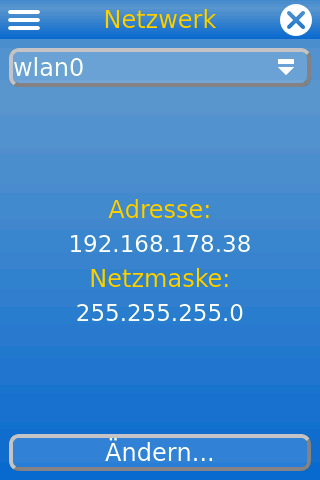
\includegraphics[scale=0.4]{images/ip-addr.png}
\caption{Anzeigen der IP-Adresse}
\end{figure}




\end{document}
